\documentclass{article}

\usepackage{listings}
\usepackage{graphicx}
\usepackage{cite}
\usepackage{url}
\usepackage{listings}
\usepackage[margin=0.5in]{geometry}

\title{BRS Readout Description}
\author{M.P.Ross}
\begin{document}
\maketitle
\section{Introduction}
This document describes the ``BRSReadout'' software which was developed by the E{\"o}t-Wash group as the readout software of the Beam Rotation Sensor (BRS). The BRS's angular readout is achieved using a multi-slit autocollimator refined from the device described in \cite{autoCol}. The goal of the software is to turn line camera images into an number of angular readout channels, which are set to the accompanying TwinCAT code, while also giving the user an interface to view the camera images, plot the angular data, record data to disk, and monitor performance. The source for BRSReadout software can be found here: \url{https://github.com/mpross/BRSReadout} or \url{slowcontrols/trunk/BRS2 C#/BRSReadout/}. The accompanying TwinCAT code can be found at \url{slowcontrols/trunk/TwinCAT3/BRS/} with a version for each BRS deployed at the observatories.

\section{Overview}
The code is split between a number of simultaneous threads to allow for increased functionality while maintaining performance. The core of the software is the Form1.cs class which analyzes the images as described in the Image Analysis section, calculates the various signals and status bits, and handles all of the data communication with other threads and the accompanying TwinCAT code. The graphing (Form2.cs), frame capturing (Camera.cs), and data writing (DataWriting.cs) are all handled in their own threads to allow the various subroutines to run at different rates while also decoupling the performance of the threads.

Upon initialization, the main loop starts the other threads, reads a collection of settings from the configuration files, and triggers the camera to begin continuous acquisition. After which is waits for a frame to come into the buffer before running the frame through the analysis, calculating signals, then sending the signals to the other threads and the TwinCAT code. It then waits for another frame and repeats until the software is closed. It should be noted that the analysis is highly CPU intensive and requires a dedicated core to achieve maximal rate while avoiding interrupts from other processes. This is achieved by utilizing the CPU Affinity setting in Windows which is set using a the AffinitySet.bat script on startup. 
\begin{center}
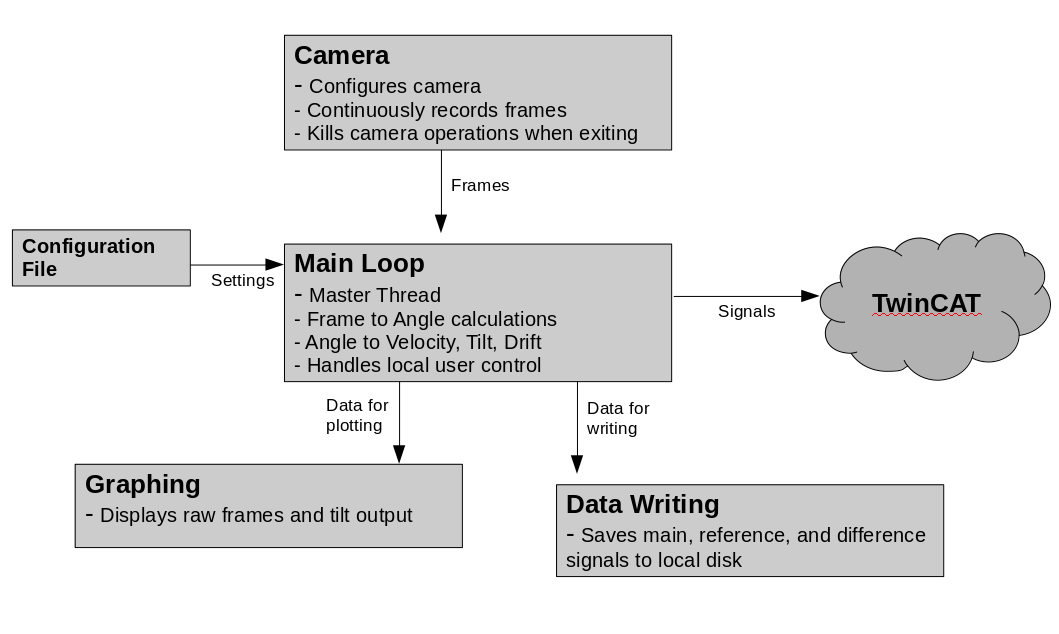
\includegraphics[width=0.75\textwidth]{BRSReadoutFlow.png}\\
\end{center}

\section{Image Analysis}
The multi-slit autocollimator shines light from a fiber coupled LED through a mask consisting of 38 slits which is then set through a beam splitter. The reflected beam is imaged onto a CCD line camera while the transmitted beam reflects off of a mirror that is attached to the beam before also being imaged on the CCD. This forms two nearly identical patterns, the reference and main patterns which respectively correspond to the reflected and transmitted path of the beam splitter. The major differences between the patterns is the height of the peaks which is due to the main pattern passing through the beam splitter twice and the spatial separation of the two patterns which is due to a static angle between the main mirror and the optical path. Introducing this static angle also reflects away the secondary reflections out of the imaging plane of the CCD.\\

\begin{center}
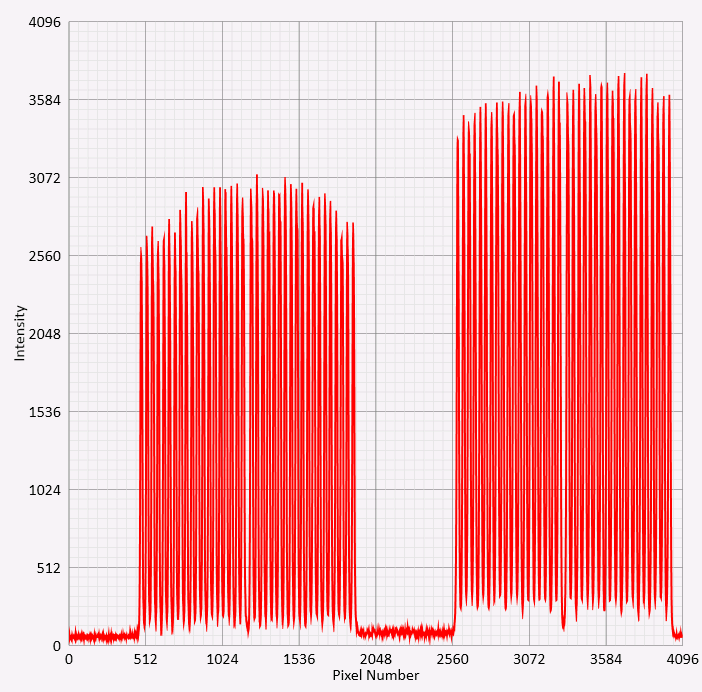
\includegraphics[width=0.5\textwidth]{BRSReadoutScreenPatterns.png}\\
\end{center}

As the angle between the beam and the housing change, the main pattern (shown above on the left) translates across the CCD while the reference pattern stays stationary. The program now needs to take these images and turn it a data stream of angular readings by measuring the distance between the patterns for each frame.

The frames are recorded by the camera as a 4096 element vector of 12 bit numbers representing the intensity of each CCD pixel. The control of the camera and initial frame handling is done in the Camera.cs class which pulls the frames from the camera using the Basler Pylon APIs, averages a small number of frames together to decrease down stream load, and puts them in a buffer to be ready by the main loop. Additionally, for some of the BRSs the cameras were intentionally installed backwards to account for which each frame is reversed before being sent on.\\

\textbf{Frame recording code Camera.startFrameGrab}:
\begin{lstlisting}{sharpc}
while (true)
{
	if (cameraType == "basler")
	{
	    PylonBuffer<Byte> buffer;
	    Pylon.WaitObjectWait(hWait, 100);

	    Pylon.StreamGrabberRetrieveResult(hGrabber, out grabResult);

	    bufferIndex = (int)grabResult.Context;

	    while (buffers.TryGetValue(grabResult.hBuffer, out buffer) != true) ;
	    Buffer.BlockCopy(buffer.Array, 0, data, 0, buffer.Array.Length);

	    if (frameReverse)
	    {
		Array.Reverse(data);
	    }
	    frameAveraging(data);
	    Pylon.StreamGrabberQueueBuffer(hGrabber, grabResult.hBuffer, bufferIndex);
	}
}
\end{lstlisting}

\section{Signal Processing}
\section{User Interface}

\begin{center}
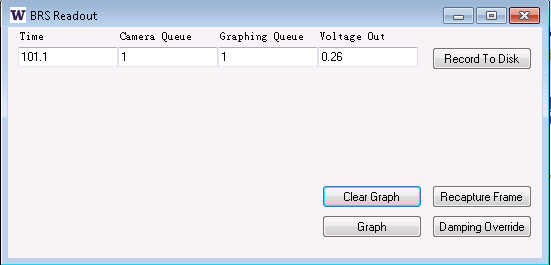
\includegraphics[width=0.5\textwidth]{BRSReadoutScreen.png}\\
\end{center}
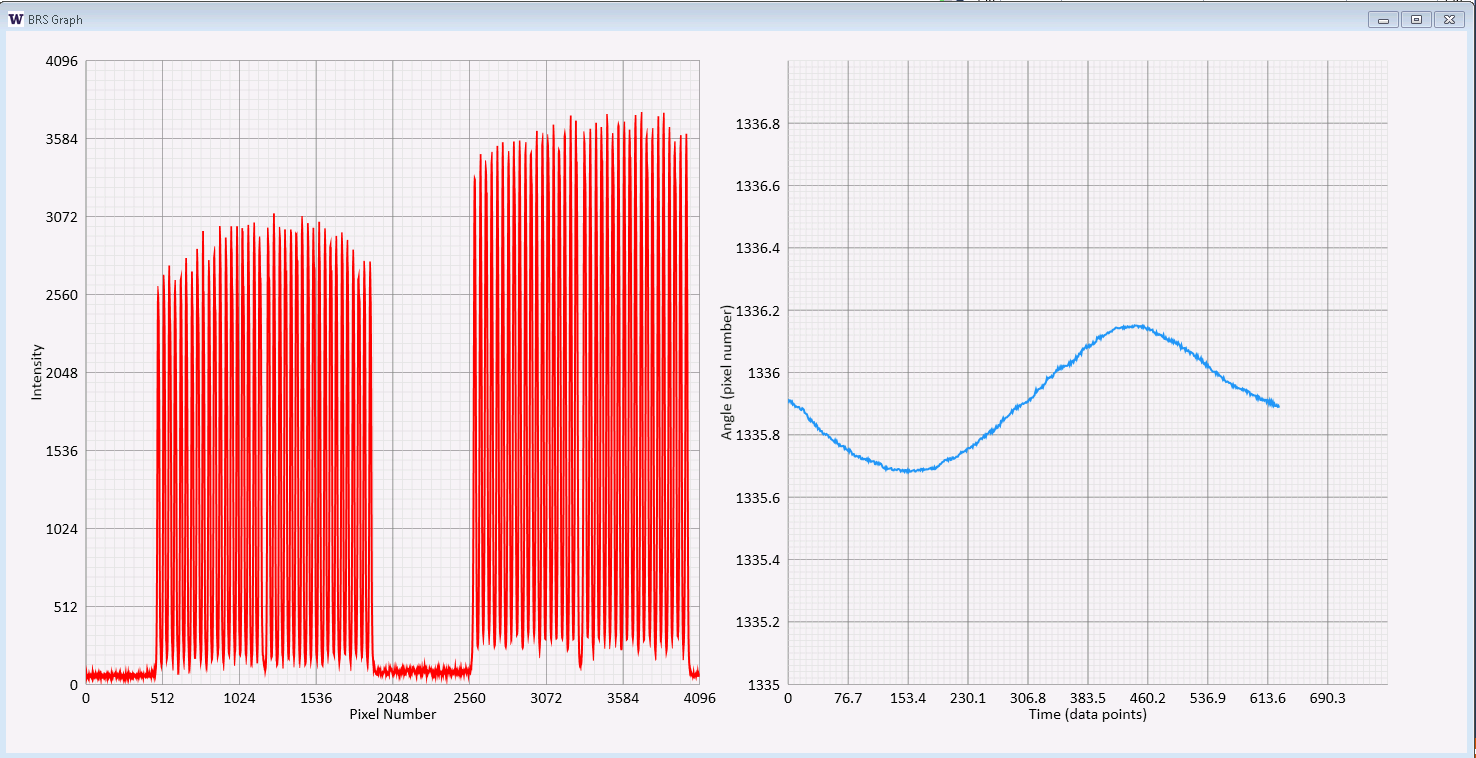
\includegraphics[width=\textwidth]{BRSReadoutScreenGraph.png}

\section{Troubleshooting}
\bibliographystyle{plain}
\bibliography{ReadoutDescription}{}
\end{document}